\documentclass[journal]{IEEEtran}

\usepackage[T1]{fontenc}
\usepackage[utf8]{inputenc}
\usepackage{lmodern}

\usepackage{ae}
% \usepackage[brazilian]{babel}
\usepackage{hyphenat}
\usepackage{fancyhdr}
\usepackage{float}
\usepackage{cite}
\usepackage[pdftex]{hyperref}
\usepackage[pdftex]{color,graphicx}

\usepackage[cmex10]{amsmath}

\usepackage{array}

\usepackage{mdwmath}
\usepackage{mdwtab}
\usepackage{url}
\usepackage{tikz}

\hyphenation{op-tical net-works semi-conduc-tor con-si-de-ram}

\begin{document}
\title{Um Estudo da Instabilidade de Saffman-Taylor com Fluido Magnético e, ou Anisotrópico}

% author names and IEEE memberships
% note positions of commas and nonbreaking spaces ( ~ ) LaTeX will not break
% a structure at a ~ so this keeps an author's name from being broken across
% two lines.
% use \thanks{} to gain access to the first footnote area
% a separate \thanks must be used for each paragraph as LaTeX2e's \thanks
% was not built to handle multiple paragraphs

\author{Ataias~Pereira~Reis, Yuri~Dumaresq~Sobral, Francisco~Ricardo~da~Cunha\\Universidade de Brasília\\Departamento de Matemática\\Brasília, Brasil\\ataiasreis@gmail.com}

% The paper headers
\markboth{ProIC, Julho~2013}%
{Shell \MakeLowercase{\textit{et al.}}: Bare Demo of IEEEtran.cls for Journals}

\maketitle


\begin{abstract}
%\boldmath
Criação de algoritmos para resolver equações diferenciais parciais. Uso de diferenças finitas para resolver as equações de Laplace e Poisson, usando método ímplicito e explícito, usando bibliotecas de álgebra linear de código aberto. Análise da diferença de tempo de resolução entre os métodos implícito e explícito. Uso do método iterativo e de resolução direta de sistema linear. 
\end{abstract}
% IEEEtran.cls defaults to using nonbold math in the Abstract.
% This preserves the distinction between vectors and scalars. However,
% if the journal you are submitting to favors bold math in the abstract,
% then you can use LaTeX's standard command \boldmath at the very start
% of the abstract to achieve this. Many IEEE journals frown on math
% in the abstract anyway.

% Note that keywords are not normally used for peerreview papers.
\begin{IEEEkeywords}
Ferrofluidos, Navier~Stokes, EDP, Poisson, Laplace, Diferenças~finitas, Eigen
\end{IEEEkeywords}

% For peer review papers, you can put extra information on the cover
% page as needed:
% \ifCLASSOPTIONpeerreview
% \begin{center} \bfseries EDICS Category: 3-BBND \end{center}
% \fi
%
% For peerreview papers, this IEEEtran command inserts a page break and
% creates the second title. It will be ignored for other modes.
\IEEEpeerreviewmaketitle

\section{Introdução}
A instabilidade de Saffman-Taylor, também chamada de endedamento, ou \textit{fingering}, é um fenômeno que ocorre na superfície de contato entre dois fluidos sob circunstâncias específicas. Esse fenômeno ocorre quando um fluido menos viscoso é injetado para deslocar um outro mais viscoso (na situação inversa, do fluido mais viscoso usado para movimentar o outro, a interface é estavel, não ocorrendo o endedamento). Também pode ocorrer movida pela gravidade, ao invés de injeção de um fluido em outro. Neste caso, a interface separando os fluidos de diferentes densidades está direcionada na horizontal, e o mais pesado está em cima do outro. Este tipo de fenômeno é um problema ocorrente em petrolíferas marítimas. Em tais petrolíferas, ocorre a injeção de água nos tubos de extração de petróleo, no objetivo do óleo subir. Na interface entre água e petróleo, o endedamento ocorre, originando bolhas de óleo dentro de água, que tem um efeito negativo na extração do petróleo, causando perca de óleo quando a água é jogada fora.

Para o estudo dessa instabilidade, que não é nada trivial, a solução se dá por meio de métodos numéricos auxiliados por computador. A equação de Navier Stokes deve ser discretizada e então resolvida numericamente. Ela é uma equação diferencial parcial altamente não-linear e de difícil resolução. No caso da instabilidade de Saffman-Taylor, no qual a fronteira está em movimento, que é a interface entre os dois fluidos, faz-se necessário algoritmos numéricos capazes de lidar com este movimento sem causar complicações extremas que impossibilitem a obtenção de soluções práticas. 

Tais ferramentas numéricas e decisão de métodos/algoritmos a se utilizar são a primeira etapa neste projeto, para então, após se ter tais ferramentas, estudar a física do problema e propor soluções para o problema com a utilização de um ferrofluido. A apresentação no resto deste relatório mostrará até onde se alcançou na codificação dos algoritmos numéricos para resolução do problema proposto, que inicia-se com o estudo de equações diferenciais parciais e de diferenças finitas na forma contínua, e só então na forma discreta. Após isso, estuda-se em específico a equação de Navier Stokes, que é dividida em etapas, para facilitar a busca de resultados.
\section{Metodologia}
A metologia aqui proposta resume as tarefas realizadas, não seguindo um ordem cronológica, mas sim uma mais organizada, para estar bem divididas as seções.
\begin{enumerate}
  \item Programação
  \item Equação de Laplace
  \item Ferramenta
  \item Método Explícito
  \item Método Implícito
  \item git e python
  \item Navier Stokes
\end{enumerate}
\subsection{Programação}
O fato do problema numérico em questão ser difícil torna o tempo uma questão fundamental na escolha da linguagem de programação a ser utilizada. De início a ferramenta e linguagem de programação utilizada era o MATLAB\textregistered. O MATLAB inclui uma infinidade de algoritmos já prontos disponíveis para uso, ferramentas para plotagem de gráficos embutidas, ótimos sistemas de referências de funções, mas tem a desvantagem de ser muito caro, proprietário e consumir muita memória e processamento só de estar aberto, sem executar o próprio programa para resolver nossas equações em questão. Como o tempo é um fator crítico, como já mencionado, o custo de memória de um programa como o MATLAB, sendo executado por muitas horas ou dias, pode ser algo muito complicado, preferiu-se tomar outro rumo para o desenvolvimento dos nossos códigos.

Tais problemas levaram a uma escolha de uma linguagem de programação compilada e rápida, o C++. O fato do aluno ter experiência em C inicialmente, aliado ao fato de se haver encontrado uma biblioteca de álgebra linear chamada Eigen que evita a necessidade de criação de inúmeros algoritmos básicos, e que é feita em C++, influenciou na escolha de tal linguagem.

A Eigen\footnote{Eigen: http://eigen.tuxfamily.org/} inclui algoritmos para resolução de sistemas lineares, criação de matrizes e alocação de memória, operações básicas de matrizes, resolução de sistemas de matrizes esparsas e vários outros algoritmos não explorados que estão à disposição, isso tudo de graça, pois é código aberto e gratuito. 

Apesar de se ter escolhido o C++ e a Eigen, isto só não traz todas as ferramentas necessárias ao trabalho em questão. A plotagem de gráficos diretamente em C++ não é algo trivial, não foram encontradas bibliotecas de fácil uso que pudessem ser utilizadas de uma forma tão simples como o MATLAB. Após muita pesquisa, foi decidido utilizar o python, e suas bibliotecas de plotagem de gráficos. Os códigos em C++ passarem a ser compilados não em programas, mas em bibliotecas, e executados de dentro do ambiente Python, bem mais leve que o MATLAB, e então com o Python, que possui poderosos recursos para salvar arquivos, plotar gráficos e tudo de fácil estudo para uso, completou-se o arsenal de ferramentas de programação que são utilizadas no presente trabalho.

Além das ferramentas que lidam direto com código, é utilizado o CMake\footnote{Cmake: http://www.cmake.org/} para criação de Makefiles para compilar o código e o git\footnote{Git: http://git-scm.com/} é utilizado como gerenciador de versões do projeto, de forma a sempre se ter as versões antigas dos códigos salvas, e bem organizadas.
\subsection{Equação de Laplace}
\subsubsection{Forma contínua}
Primeiramente, teve-se a familiarização do aluno com a resolução de equações diferenciais parciais, realizando um curso na UnB, onde foram vistas principalmente a equação de Laplace, Poisson, Calor e Onda. O método de resolução aprendido foi por separação de variáveis, o método de Fourier. Após isso, o primeiro problema proposto foi resolver uma destas equações numericamente, a escolhida foi a equação de Laplace em duas dimensões, que segue abaixo:
\begin{equation}
\nabla^2 u=\frac{\partial^2 u}{\partial x^2}+\frac{\partial^2 u}{\partial y^2}=0\label{laplace}
\end{equation}

A primeira etapa na resolução desta equação de maneira numérica é discretizá-la, e isto quer dizer limitar o domínio, escolher um número de pontos em cada dimensão, e representar a equação como operações mais simples que o computador possa entender, diferentes da derivada. O escolhido foi utilizar as diferenças finitas.
\subsubsection{Forma discreta - explícito}
Para a discretização da equação \ref{laplace}, usa-se o método mencionado antes, que são as diferenças finitas. Este método basicamente faz a seguinte aproximação para a derivada:
\begin{equation}
f'(x)=\lim_{h\rightarrow 0}\frac{f(x+h)-f(x)}{h}=\frac{d}{dx}f(x)\approx \frac{f_i-f_{i-1}}{\Delta x}
\end{equation}
Os valores de $f_i$ são valores discretizados da função $f(x)$, ou seja, $f_i=f(i\Delta x)$. Agora a distância entre dois pontos passa a ser de $\Delta x$, e daí a derivada se calcula como a diferença entre um ponto e outro, dividida pela distância entre eles. Há vários tipos de diferenças: progressivas, regressivas, centrais e podem ter mais pontos, e diferentes ordens de erro podem ser obtidas dependendo dos valores de $\Delta x$ e do número de pontos usados nos cálculos. Para Laplace, utilizou-se diferenças centrais de segunda ordem. Neste caso, o erro é da ordem de $\Delta x^2$.
\begin{equation}
f''(x)\approx \frac{f(x+\Delta x)-2f(x)-f(x-\Delta x)}{\Delta x^2}
\end{equation}
Utilizando essa equação para laplace, chegamos na seguinte discretização, considerando $\Delta x=\Delta y$ e que a variável $x$ varia com pontos indicados pelo indice $i$ e a variável $y$ com o índice $j$:
\begin{equation}
\frac{u_{i+1j}+u_{i-1j}+u_{ij+1}+u_{ij-1}-4u_{ij}}{\Delta x^2}=0
\end{equation}
Reordenando essa equação:
\begin{equation}
  u_{ij}=\frac{u_{i+1j}+u_{i-1j}+u_{ij+1}+u_{ij-1}}{4} \label{laplace_discreta}
\end{equation}
\subsubsection{Domínio}
A equação da fórmula \ref{laplace_discreta} está na forma explícita, na qual um ponto se obtém a partir de outros pontos, mas como quando se muda o valor de um ponto, ele influencia no cálculo de outros, esta fórmula deve ser aplicada muitas vezes, até se alcançar a convergência em todos os pontos do domínio. Entretanto, se apenas aplica-se essa equação a todos os pontos do domínio, já se vê um problema, pois ela sempre pede mais pontos para os lados. Por isso, além da equação, necessita-se das condições de contorno para o problema, onde-se são determinados os valores nas fronteiras do domínio, de forma direta ou indireta, dependendo se as condições são de Dirichlet, Neumann ou uma mistura. O domínio escolhido é um quadrado, e abaixo tem-se o exemplo de uma malha 6x6.

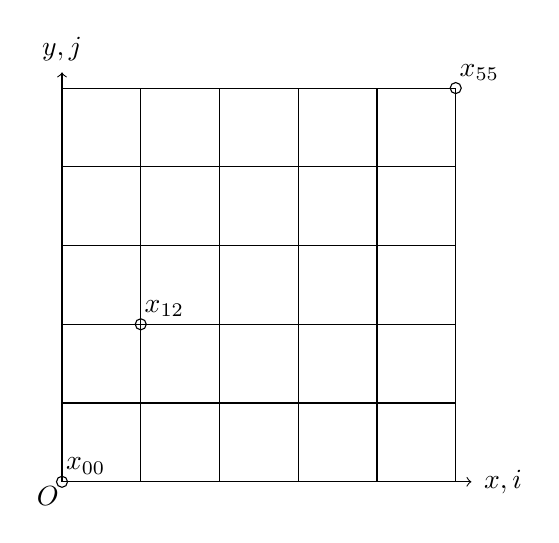
\begin{tikzpicture}
%grid
\draw (0,0) grid +(5,5);

%axes
\draw[->] (0,0) -- (xyz cs:x=0, y=5.2);
\draw (0,5.5) node {$y,j$};

\draw[->] (0,0) -- (xyz cs:x=5.2,y=0);
\draw (5.6,0) node {$x,i$};
\draw (-0.18,-0.18) node {$O$};

\draw (0.3,0.2) node {$x_{00}$};
\draw (0,0) circle (2pt);

\draw (5.3,5.2) node {$x_{55}$};
\draw (5,5) circle (2pt);

\draw (1.3,2.2) node {$x_{12}$};
\draw (1,2) circle (2pt);
\end{tikzpicture}

Cada cruzamento de linha indica um ponto no domínio, e a equação \ref{laplace_discreta} será aplicada em quase todos estes postos, com exceção dos de fronteira. O valor dos pontos de fronteira deste primeiro problema foi escolhido fixo, utilizando condições de Dirichlet. 

Pelo fato do método ser iterativo, com um \textit{loop} sendo repetido muitas vezes, até a convergência, é natural escolher um método de parada. Isto poderia ser escolher um tempo limite de execução, ou ver a diferença entre duas matrizes após uma iteração completa em seus pontos internos, para analisar se a diferença entre elas é desprezível e se pode mudar o valor, ou ainda calcular os valores das derivadas nos pontos, que seria o melhor a se fazer, e analisar se a equação está dentro de uma faixa de erro desejada. A segunda maneira de se fazer isto foi escolhida na primeira parte, e foi difícil escolher qual utilizar, pois ainda não se via a diferença que poderia ter entre os dois últimos, principalmente, ou não se pensava claramente como por o último em prática.
\section{Resultados}
\subsection{Laplace - Método Iterativo}
Foram realizados vários testes utilizando as seguintes condições:
\begin{eqnarray}
\nabla^2 u=0\\
u_{}
\end{eqnarray}
\newpage
\subsection{Programas\label{exemplos}}
\newpage

\subsection{Acessar dois Kinects}


\section{Conclusão}

% use section* for acknowledgement
\section*{Agradecimentos}


The authors would like to thank...

\begin{thebibliography}{4}
  
\bibitem{ubuntu} \href{ftp://ftp.fisio.cinvestav.mx/Manuales/linux/Getting\%20Started\%20with\%20Ubuntu\%2010.10.pdf}{Getting Started with Ubuntu 10.10}
\bibitem{openkinect} \href{http://openkinect.org/wiki/Main_Page}{OpenKinect}
\end{thebibliography}
\end{document}
